\section{Introduction}

\begin{frame}
\tableofcontents[currentsection, hideothersubsections]
\end{frame}

\begin{frame}{Problématique}
	\begin{alertblock}{AVC : Constat}
		Un individu sur 600 est victime d'un AVC chaque année. \\
		120 000 AVC/an en France. \\ \pause 
		Cause fréquente d'hémiplégie chez les victimes. \\
		Une des principales causes d'invalidité.
	\end{alertblock}
\end{frame}

\begin{frame}
	\begin{block}{Réponse actuelle}
	Des programmes de réhabilitations.\\
	Des tests de mesure des capacités sensorimotrices :
		\begin{itemize}
			\item Tests de déficience
			\item Tests fonctionnels
		\end{itemize}
	\end{block}

\begin{block}{Les standards actuels}
Un test de déficience: le score de Fugl Meyer \\
Un instrument de mesure des angles : le goniomètre
\end{block}
\begin{center}
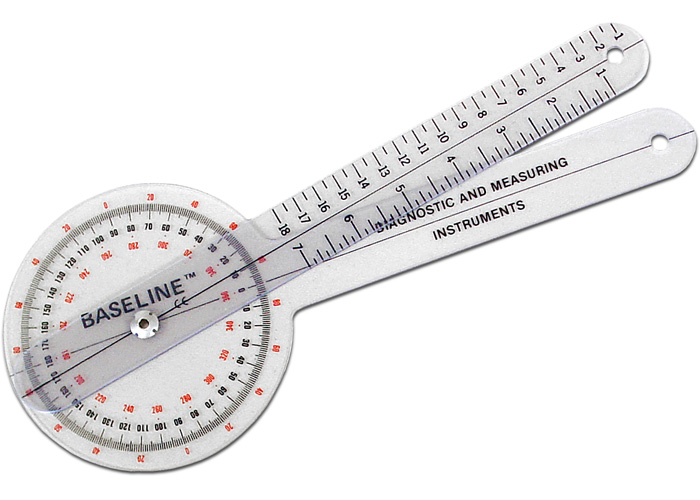
\includegraphics[width=3.8cm]{../images/goniometre.jpg}
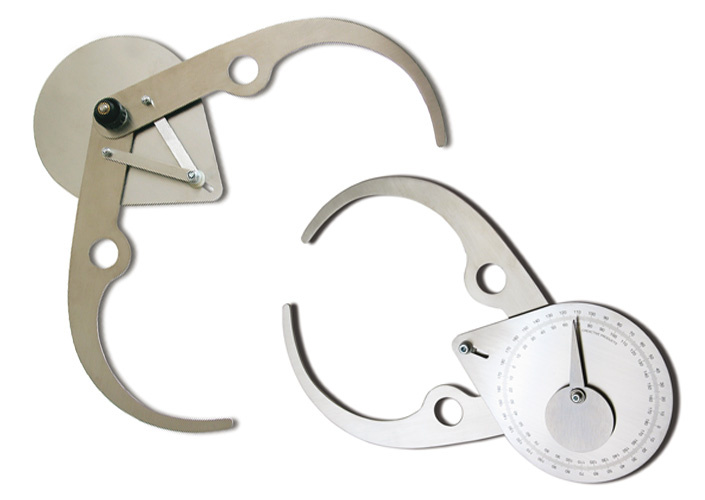
\includegraphics[width=3.7cm]{../images/clockprop.jpg}
\end{center}
\end{frame}

\begin{frame}
\begin{block}{Limites}
Le test de FM nécessite des mesures d'angles précises.\\
Repérer des mouvements \textit{illégaux} \\ \pause
Le goniomètre se révèle :
\begin{itemize}
	\item intrusif
	\item imprécis
	\item finalement souvent délaissé
\end{itemize}
\end{block}
\end{frame}
